% Citations with year
\documentclass[msc,proposal,hideapproval,hidededication,hideack,
               hideepigraph,hidelof,hidelot,hideabstract]{ppgccufmg} 
\usepackage[english]{babel}
\usepackage[latin1]{inputenc}
\usepackage[T1]{fontenc}
\usepackage{type1ec}
\usepackage{graphicx}
\usepackage[a4paper,
  portuguese,
  bookmarks=true,
  bookmarksnumbered=true,
  linktocpage,
  colorlinks,
  citecolor=black,
  urlcolor=black,
  linkcolor=black,
  filecolor=black,
  ]{hyperref}
\usepackage{tabularx}
\usepackage{scalerel}
\usepackage[square,numbers]{natbib}
\usepackage[dvipsnames]{xcolor}

\begin{document}
%\let\cleardoublepage\clearpage % ALBERTO

\ppgccufmg{
  title={Finding References of Reputation},
  authorrev={Ueda, Alberto Hideki},
  university={Federal University of Minas Gerais},
  course={Computer Science},
  portuguesetitle={Finding References of Reputation},
  portugueseuniversity={Universidade Federal de Minas Gerais},
  portuguesecourse={Ci�ncia da Computa��o},
  address={Belo Horizonte},
  date={2016-04},
  advisor={Berthier Ribeiro-Neto},
  coadvisor={N�vio Ziviani  
  \\ Rodrygo L. T. Santos},
  abstract={Abstract}{abstract},%    \keywords{Computer Vision, Networks, Sabotage}
}

\chapter{Introduction}

\section{What is Reputation?}

% What is Reputation? % Why is it important? % Examples
Reputation is a widespread notion in society, albeit an arguably ill-defined one. In general, the reputation of an entity reflects the public perception about this entity developed over time \citep{ribas2015random}. This public perception may be either good or bad, and touches a variety of aspects that may impact the identity of the entity before the public, such as its competence, integrity and trustworthiness. Moreover, the reputation of an entity can change rapidly following an event in which the entity is involved, by means of word-of-mouth dissemination -- whether traditional or electronic. As a result, reputation has been subject of professional management by public relations departments as well as of collective management by members of online communities, such as question-answering forums and online marketplaces \citep{hutton2001prr}.

% Why is it challenging?
The identification of reputable entities is an important task in many fields. Indeed, more reputable entities are presumably a better fit for most purposes. However, the subjective nature of reputation makes its quantification -- and hence the identification of reputable entities -- challenging. As a result, existing attempts to quantify the reputation of an entity rely on either manual assessments or on a restrictive definition of reputation, e.g., in terms of authority~\cite{kleinberg98,page98pagerank}, influence~\cite{bakshy2012www}, or expertise~\cite{balog2012ftir}. 

In this work, we take an agnostic view of reputation. In particular, instead of relying on a single, precise definition of reputation, we exploit the \textit{transference} of reputation among entities in order to identify the most reputable ones.

\section{An Academic Example}

% How reputation applies in academia?
For instance, evaluating a group of researchers is a permanent problem within research and academic institutions, laboratories and funding agencies \cite{lima2013jcdl}. Usually, this process involves forming highly qualified committees that must meet, define evaluation criteria and perform the evaluation. Moreover, it is very costly in terms of time, because evaluating numerous researchers (their curricula and publications) is not a simple process.

% How is it measured today? % Why the reputation matters in academia?
The decision of which researchers should be at the top -- for hiring, promoting, funding, or distributing grants, scholarships, awards and so on -- is typically based on criteria such as number of publications, impact of publications, number of undergraduate and graduate students under supervision, number of advised MSc and PhD theses, and participation in committees (conferences, journal editorial boards, technical committees, etc). Clearly, the effectiveness of the resulting ranking depends on how each criterion is assessed and the period of time covered in the assessment. Several indices have become widely used to measure the productivity of researchers. Examples include the raw number of citations, h-index ~\cite{hirsch2005}, g-index \cite{egghe2006theory} and citation z-score \cite{zscore}. Likewise, most academic search platforms, such as Google Scholar\footnote{\url{http://scholar.google.com}}, Microsoft Academic Search\footnote{\url{http://academic.research.microsoft.com}} and ArnetMiner\footnote{\url{http://arnetminer.org}}, use some of such indices to rank researchers.

% Who are the entitites?
The same problem -- finding the top academic entities -- applies to the context of research groups, departments, universities and publication venues (conferences and journals). The general nature of the problem and the different relationships between the entities motivate us to use network analysis techniques as random walks and clustering. 

For illustrative purposes, let us show the distribution of Brazilian researchers according to CNPq productivity levels in Computer Science, in Table~\ref{tab:cnpq-levels}. This distribution is the result of an evaluation process quite similar to that described in the first paragraphs of this section. The table shows that there are just 390 CS researchers in all of the Brazil, out of many thousands, who receive an individual research grant from CNPq.
%
To compute this distribution, an important rule is applied: regardless the metric used to rank researchers, there is a percentage limit for the number of authors in each productivity level, except the last one (level 2). This limitation applies to the whole area of Computer Science, without considering the specificities of each of its sub-areas. One can see that independently of the academic metrics used, some sub-areas of Computer Science have intrinsic disadvantages in this classification. This problem motivates the current work and it is best addressed in next section.

% sabir@ultrasr:~/Develop/rscore-workspace/rscore_mongo/person$ cat bolsistas_produtividade.tsv | awk '{print $2}' | sort | uniq -c
\begin{table}[h]
\centering \small
\caption{Distribution of researchers in CNPq productivity levels in Computer Science (CS) and in all areas of science}
\label{tab:cnpq-levels}
\begin{tabular}{ccc}
\\
\toprule
Level & \multicolumn{2}{c}{Researchers} \\ %\cline{2-3}
      & CS & All Areas \\ 
\midrule
%SR   & 0 & 91 \\
1A &  23 (5.9\%) & 1320 (9.2\%) \\
1B &  22 (5.6\%) & 1308 (9.1\%) \\
1C &  31 (7.9\%) & 1376 (9.6\%) \\
1D &  70 (17.9\%) & 2386 (16.7\%) \\
2  & 244 (62.6\%) & 7933 (55.4\%) \\
\midrule
%Total & 390 & 14414 \\ % with SR
Total & 390 & 14,323 \\ % without SR
\bottomrule
\end{tabular}
\end{table}



%%%%%%%%%%%%%%%%%%%%%%%%%%%%%%%%%%%%%%%%%%%%%%%%%%%%%%%%%%%%%%%%%%%%%%%%%%%%%%%%%%%%%%
\section{What Do We Propose?}

% What are the problems of the current approaches? What are the limitations?
Ranking researchers without regarding the specificity of their areas or sub-fields of research is arguably unfair and potentially error-prone \cite{lima2013jcdl}. For instance, consider the area of Human-Computer Interaction within the broad field of Computer Science (CS) [2]. Experimental evaluation in this area usually takes more time than in other CS areas when arranging and assessing users' feedback is necessary. On the other hand, CS areas such as Databases and Computer Graphics do not usually face the same problem because their experimental evaluations depend on assessing the outcome of an automatic process, such as a query evaluation or a graphics rendering engine. Likewise, researchers from some areas may have fewer publications than others, but with a potentially higher impact in their community.

In order to have a better understanding of this current problem in academic rankings, see the scenario of Computer Science in Table \ref{tab:subareas}.  It contains a list of 24 sub-areas of Computer Science according to Microsoft Academic Search.

% Problem 
% 24 subareas
\begin{table}[h]
\caption{Sub-areas of Computer Science according to Microsoft Academic Search} % d=1 (contagem)
\label{tab:subareas}
\small \centering
%\setlength{\tabcolsep}{3pt}
\begin{tabular}{cl}
 & \\
\toprule
\#  & Subarea \\
\midrule
1 & Algorithms \& Theory \\ 
2 & Artificial Intelligence \\ 
3 & Bioinformatics \& Computational Biology \\ 
4 & Computer Vision \\ 
5 & Data Mining \\ 
6 & Databases \\ 
7 & Distributed \& Parallel Computing \\ 
8 & Graphics \\ 
9 & Hardware \& Architecture \\ 
10 & Human-Computer Interaction \\ 
11 & Information Retrieval \\ 
12 & Machine Learning \& Pattern Recognition \\ 
13 & Multimedia \\ 
14 & Natural Language \& Speech \\ 
15 & Networks \& Communications \\ 
17 & Operating Systems \\ 
18 & Programming Languages \\ 
19 & Real-Time \& Embedded Systems \\ 
20 & Scientific Computing \\ 
21 & Security \& Privacy \\ 
22 & Simulation \\ 
23 & Software Engineering \\ 
24 & World Wide Web\\
\bottomrule
\end{tabular}
\end{table}

% Brazil Qualis (Theory, BD)
In several academic communities, Brazilian researchers included, the distribution of grants, scholarships, awards, productivity levels, among others, are computed from the perspective of the whole area of Computer Science. Further, funding agencies as the \textit{Conselho Nacional de Pesquisa (CNPq)} impose numerical limits on the members of grants issued to any given broad area of knowledge such as Computer Science. It so, one can realize that the most popular sub-areas in Computer Science have large advantages in this classification process over the other sub-areas in CS. For instance, the sub-area of computational theory cannot be equally compared to data mining, since the latter has more researchers, publications, and venues available today than the former one. Therefore, there is a necessity of a closer look to these academic scenarios from a perspective of sub-areas.

% In addition, we demonstrate the robustness of our model to random perturbations in the selection of reputation sources, and the suitability of semi-automatically choosing effective reputation sources using the model itself.
\pagebreak
One of the goals of this work is to find a fair and trustworthy way to rebalance these academic rankings in the context of sub-areas. To do that, we intend to use different approaches and modern metrics of relevance, including a generic model of reputation called P-score, which we describe in Chapter 2. 

Some of the research questions we want to answer are: i) How to be fair with small sub-areas of knowledge or sub-areas with a low frequency of publications considering scientific impact categorization? ii) How well Brazilian research groups are internationally doing from the perspective of sub-areas? iii) How to characterize sub-areas in terms of scientific impact? iv) Can we find groups with the highest reputation in any topic of knowledge only adjusting the input data, but using the same method for sub-areas?

%%%%%%%%%%%%%%%%%%%%%%%%%%%%%%%%%%%%%%%%%%%%%%%%%%%%%%%%%%%%%%%%%%%%%%%%%%%%%%%%
\chapter{Related Work}

% Reverse
In this section, we review the related literature on ranking based on random walks, as well as approaches devoted to generating rankings in an academic search setting.

\section{Ranking in Academic Search}

% Initial Rankings
Ranking has traditionally played an important role in academic search, particularly for tasks related to assessing the scientific productivity of academic entities. In particular, one of the earliest metrics proposed to quantify academic impact was Garfield's Impact Factor~\cite{garfield1955}. Despite its wide usage since it was proposed in 1955, it has been largely criticized~\cite{saha2003}. As a result, many alternatives have been proposed in the literature, such as other citation-based metrics like the H-Index~\cite{hirsch2005}, download-based metrics~\cite{bollen2005toward}, and PageRank-like metrics~\cite{Yan:2007}. As argued by Leydesdorff~\cite{leydesdorff2009new}, each metric has its own bias and there are both advantages and disadvantages associated with each one.

% Citations
Citation-based metrics have been applied to rank computer and information science journals~\cite{Katerattanakul2003,nerur2005assessing}. Also, several citation-based metrics have been proposed to measure the quality of a small set of conferences and journals in the database field~\cite{rahm2005citation}, and to rank documents retrieved from a digital library~\cite{larsen2006using}. Mann et al.~\cite{Mann:2006} introduced topic modeling to further complement the citation-based bibliometric indicators, producing more fine-grained impact measures. Yan and Lee~\cite{Yan:2007} proposed two measures for ranking the impact of academic venues which aim at efficiency and at mimicking the results of the widely accepted Impact Factor. An alternative method was presented by Zhuang et al.~\cite{Zhuang:2007}, who proposed a set of heuristics to automatically discover prestigious and low-quality conferences by mining the characteristics of program committee members.

% Beyond citations
Piwowar~\cite{piwowar2013altmetrics} recently claimed that citation-based metrics are useful, but not sufficient to evaluate research. In particular, he observed that metrics like the H-Index are slow. Indeed, the first citation of a scientific article can take years. As a result, he argued for the development of alternative metrics to complement citation analysis. In a similar vein, Lima et al.~\cite{lima2013jcdl} argued that productivity indices should account for the singularities of the publication patterns of different research areas, in order to produce an unbiased assessment of the impact of academic output. Accordingly, they proposed to assess a researcher's productivity by aggregating his or her impact indicators across multiple areas. Finally, Gon�alves et al.~\cite{goncalves2014} investigated the importance of various academic features to scholar popularity and concluded that only two features are needed to explain all the variation in popularity across different scholars: (i) the number of publications and (ii) the average quality of the scholar's publication venues. The metric P-score -- one of the methods used in this work -- exploits exactly these two features to rank different venues and different researchers.

% Reputation
The idea of reputation, instead of citations, was discussed by Nelakuditi et al.~\cite{nelakuditi2011snap}. In particular, they proposed a metric called peers' reputation, which measures the selectivity of a publication venue based upon the reputation of its authors' institutions. The proposed metric was shown to be a better indicator of selectivity than the acceptance ratio. In addition, the authors observed that many conferences have similar or better peers' reputation than journals. Another approach related to ours was proposed by Cormode et al.~\cite{cormode2014people}, who attempted to rank authors according to their similarity with respect to a reference author. 
%In contrast to that approach, we use a strategy that allows for multiple entities -- as opposed to a single one -- to serve as a source of reputation. More importantly, instead of identifying similar entities from whom to propagate reputation, we explore the notion of reputation sources as part of a stochastic Markov process. As a result, our approach is able to produce a global reputation-oriented ranking of multiple interconnected entities.

% Laender sigs-graph Clustering
Alves et al. \cite{alves} and Lima et al. \cite{laendersigs} analyze the structure of the communities formed by the flagship conferences of ACM SIGs. Their findings show that most of the ACM SIGs are able to connect their main authors in large and visually well-structured communities. However, they note that a few conferences, such as the ACM Symposium on Applied Computing, flagship conference of SIGAPP, and the ACM Conference on Design of Communications, flagship conference of SIGDOC, do not form a strong research community, presenting a structure with several disconnected components. They have opened their results to the research community as an interactive visualization tool\footnote{\url{http://acmsig-communities.dcc.ufmg.br}} that allows one to browse the scientific communities, visualizing their structures and the contribution of each specific researcher to connect its coauthorship graph. The concept of scientific community and its natural development has enforced the clustering approach we adopt in this work.

\section{Ranking with Random Walks}

Random walks have been widely used in information retrieval. They allow us to produce rankings of interconnected entities in a network, highlighting the most important nodes from a structural perspective. Page and Brin~\cite{page98pagerank} designed the PageRank algorithm to calculate the importance of pages on the Web. PageRank simulates a web surfer's behavior. In particular, with probability $p < 1$, the surfer randomly chooses one of the hyperlinks of the current page and jumps to the page it links to; otherwise, with probability $1 - p$, the user jumps to a web page chosen uniformly at random from the collection. This defines a Markov chain on the web graph, where each probability of the stationary distribution corresponds to the rank of a web page, referred to as its {\em pagerank}.

Kleinberg~\cite{kleinberg98} divided the notion of ``importance" of a webpage into two related attributes: {\em hub}, measured by the authority score of other pages that the page links to, and {\em authority}, measured by the hub score of the pages that link to the page. These attributes are calculated in his Hyperlinked-Induced Topic Search (HITS) algorithm. Both algorithms, PageRank and HITS, have been successfully applied to rank the importance of different web pages through analyzing the link structure of the web graph.

% Extensions of the models
Extensions of the random walk model were also studied for scoring several types of objects -- e.g., products, people, and organizations -- in different applications. For instance, Nie et al.~\cite{nie05webobjects} presented PopRank, a domain-independent object-level link analysis model to rank objects within a specific domain, by assigning a popularity propagation factor to each type of object relationship. Different popularity propagation factors for these heterogeneous relationships were assessed with respect to their impact on the global popularity ranking. Xi et al.~\cite{xi04fusion} proposed a unified link analysis framework, called Link Fusion, which considers two different categories of links: intra-type links, which represent the relationship of data objects of a homogeneous data type (e.g., web pages), and inter-type links, which represent the relationship of data objects of different data types (e.g., between users and web pages). Regarding the recommendation of generic types of object, Jamali and Ester~\cite{jamali09trustwalker} proposed TrustWalker, a random walk method that combines trust-based and item-based recommendation, considering not only ratings of the target item, but also those of similar items.

% Social Networks and influencers 
Under the context of social networking systems, social friendship and random walks have been shown to be beneficial for collaborative filtering-based recommendation systems. These works argue that social friends -- for instance, in Facebook or Twitter -- tend to share common interests and thus their relationships should be considered in the process of collaborative filtering~\cite{ye11poi}. In this context, a random walk sees a social network as a graph with probabilistically weighted links that represent social relations and thus is able to accurately predict users' preferences to items and their social influence with respect to other users. Backstrom and Leskovec~\cite{backstrom11social} proposed an algorithm based on supervised random walks that combines the information from the network structure with node and edge level attributes, using these attributes to guide the random walk on the graph. 

\section{Random Walks in Academic Search}

Earlier works have studied the application of random walks for ranking authors, papers, and venues in an academic setting. For instance, Sun and Giles~\cite{sun2007popularity} proposed a popularity weighted ranking algorithm for academic digital libraries that uses the popularity factor of a publication venue. Their approach overcomes some limitations of the Impact Factor and performs better than PageRank, citation counting, and HITS. Relatedly, Zhou et al.~\cite{zhou2007co} proposed a method for co-ranking authors and their publications using several networks. Similarly, Yan et al.~\cite{yan2011p} presented a new informetric indicator, P-Rank, for measuring prestige in heterogeneous scholarly networks containing articles, authors, and journals. P-Rank differentiates the weight of each citation based on its citing papers, citing journals and citing authors.

In a narrower perspective, random walks have also been used for the task of expert finding in academic search collections. For instance, Deng et al.~\cite{deng2012modeling} proposed a joint regularization framework to enhance expertise retrieval in academia by modeling heterogeneous networks as regularization constraints on top of a document-centric model~\cite{balog2012ftir}. Relatedly, Wu et al.~\cite{wu2009detecting} proposed to model authors and publications as nodes of a publication network, with additional edges representing co-authorship information (author-author edges). In a similar vein, Tang et al.~\cite{tang2008topic} proposed a probabilistic topic modeling approach to enrich a heterogeneous graph comprising multiple academic entities as nodes, including authors, papers, and publication venues, with directed edges representing a variety of relationships such as ``written by'' and ``published in''. The stationary distribution computed after a random walk on this graph was then used to rank these entities with respect to an input query. A very similar approach was proposed by Gollapalli et al.~\cite{gollapalli2011ranking}, by assigning topics to nodes and then computing the unique stationary distribution of the associated Markov chain.

% Finding Experts

\subsection*{Reputation Flows}

In contrast to the aforementioned works, we use random walks to model the \textit{transference} of reputation from \textit{multiple} reference sources to selected targets in a reputation graph, as discussed in our previous work \cite{ribas2015random}. In order to validate our model, we instantiated it in an academic search setting by using research groups as reputation sources and publication venues as reputation targets. Moreover, while previous approaches have exploited multiple ranking signals, we demonstrated the power of the notion of reputation transfer by relying on publishing behavior as the only reputation signal.

% ICTIR
% proposal: reputation emanates from selected sources
Here we briefly discuss the instantiation of our conceptual framework of {\em reputation flows} in the academic context to model the transference of reputation between authors, papers, research groups and publication venues. The relations between these scientific entities may be captured through distinct metrics and, as far as we know, the most important ones (including citation-based metrics) fit well in our conceptual framework. In our experiments, we study how the reputation of a reference set of research groups is propagated to the venues they publish in and to other individual researchers by applying the concept of reputation flows. In this conceptual framework, publication venues are aggregations of papers and research groups are aggregations of authors, as shown in Figure~\ref{fig:groups-venues}. These aggregations are sufficient to establish core relations that allow ranking these entities.

\begin{figure}[h]
  \centering \small
  \def\x{\begin{array}{c}x\\x\end{array}}
  \(
  \let\svarraycolsep\arraycolsep
  \renewcommand\arraystretch{1.4}
  \begin{array}{c}
   \\
   {\scriptstyle Group}\\
   {\scriptstyle Venue}\\
  \\
  \end{array}
  \begin{array}{c}
   \\
   \scalerel*[1.5ex]{[}{\x}\\
  \\
  \end{array}
  \begin{array}{c}
   {\scriptstyle Group}\\
   Group \rightarrow Group \\
   Venue  \rightarrow Group \\
  \\
  \end{array}
  \begin{array}{c}
   {\scriptstyle Venue}\\
   Group  \rightarrow Venue \\
   Venue   \rightarrow Venue \\
  \\
  \end{array}
  \begin{array}{c}
   \\
   \scalerel*[1.5ex]{]}{\x}\\
  \\
  \end{array}
  \mathrm{}
  \arraycolsep\svarraycolsep
  \renewcommand\arraystretch{1.0}
  \)
  %\vspace{-0.6cm}
  \caption{Reputation flows between groups and venues.}
  \label{fig:groups-venues}
\end{figure}

% Pscore
The basic idea of the P-score metric is to associate a reputation with publication venues based on the publication patterns of a {\em reference set} of research groups in a given area or sub-area of knowledge. Given a pre-selected set of reference research groups, P-score associates weights with the publication venues the researchers in the reference groups publish in. Further, these weights can be used to rank other research groups or authors. 

The reputation of a research group is strongly influenced by the reputation of its members, which is largely dependent on their publication records. We assume that i) A research group conveys reputation to a publication venue proportionally to its own reputation, and ii) A publication venue conveys reputation to a research group proportionally to its own reputation. Once a reference group is selected, the reputation of its members is transferred to the venues. Recursively, since the reputation of research groups is correlated with the reputation of the venues in which they published, the venues transfer reputation to the groups. We use these hypotheses to build a Markov chain in which the nodes are research groups and publication venues. This chain can be solved by a stochastic computation which associates steady state probabilities to each node in the chain. These probabilities are taken as weights associated with venues which we refer to as P-scores.

% contributions
In summary, the main contributions of this previous work are i) a novel random walk model for ranking entities according to the reputation collectively transferred to them by other entities in a reputation graph; b) an empirical validation of the effectiveness and robustness of the proposed model for two academic search tasks, namely, venue and researcher ranking; c) a preliminary investigation of the suitability of automatically choosing effective reputation sources. One of the goals of our current work aims to study and propose improvements for the latter item, i.e., the selection of academic entities -- venues, researchers or research groups -- as reputation sources \cite{ribas2015bigscholar}.

\chapter{Methodology}

In this chapter we describe the datasets we will use in this work, some initial experiments we have already done, the next studies we intend to perform and a time schedule for the main tasks of this research.

\section{Datasets}

\subsection*{DBLP} 

We have a collection of scientific publications extracted from DBLP \cite{ley}, a digital library containing more than 3 million publications from more than 1.5 million authors that provides bibliographic information on major computer science conference proceedings and journals\footnote{\url{http://dblp.uni-trier.de}}. Each publication is accompanied by its title, list of authors, year of publication, and publication venue, i.e., conference or journal. 

\subsection*{Microsoft Academic Graph}

The Microsoft Academic Graph\footnote{\url{http://research.microsoft.com/en-us/projects/mag/}} (MAG) is a heterogeneous graph containing scientific publication records, citation relationships between publications -- as well as authors, institutions, journals, conferences, and fields of study. It contains individual information about more than 120 million papers.

% V E = 49870036 952364264
In Table~\ref{tab:dataset}, we present some statistics of the MAG dataset that are relevant to this work. Notice that a large fraction (59\%) of the papers in this dataset have no information on citations, that is, the paper can be represented as a node in the citation graph that has neither inlinks nor outlinks. There are two possible reasons for this to happen. The first alternative is the zero degree (i.e., both in- and out-degree) is a true representation of reality, it is a paper that in fact does not receive any citation yet and does not cite any other paper. The second alternative is due to the fact that any big repository offers an approximation of the reality, which also happens in the MAG dataset. Collecting and organizing a real-world dataset of such size is not a trivial task. In fact, it is a process that involves the treatment of huge amounts of semi-structured data, which usually causes  inconsistencies. This lack of information reinforces the necessity of alternative strategies to citation-based methods.

\begin{table}[htbp]
\centering
\caption{Relevant statistics on the Microsoft Academic Graph}
\begin{tabular}{|l|r|}
\hline
Papers with citation information    &  49,870,036 \\ \hline
Papers without citation information &  71,017,797 \\ \hline
Total number of papers              & 120,887,833 \\ \hline
\end{tabular}
\label{tab:dataset}
\end{table}


\section{Experiments}

% Clustering
Initially, we explored some clustering methods in order to help us characterize research communities. To do that, we built a graph of coauthorships, using the data from the DBLP dataset. In this graph, each node is a distinct researcher and each edge represents a cowork of the authors -- an article written by the both authors. The higher the number of collaborations between the authors, the greater the weight of the edge connecting them. We use this weight as a measure of collaboration among the authors. This allows us to run clustering algorithms and analyze the resulting communities, as we now discuss.

\subsection{Markov Cluster Algorithm}

One of the main algorithms used in our initial studies, the Markov Cluster Algorithm (MCL) discussed in \cite{mcl} is a fast and scalable unsupervised cluster algorithm for graphs based on simulation of stochastic flow in graphs. It finds cluster structures in graphs by a mathematical bootstrapping procedure. The process deterministically computes (the probabilities of) random walks through the graph, and uses two operators transforming one set of probabilities into another. It does so using the language of stochastic matrices (also called Markov matrices) which capture the mathematical concept of random walks on a graph.
The MCL algorithm simulates random walks within a graph by an alternation of two operators called expansion and inflation. The expansion coincides with taking the power of a stochastic matrix using the normal matrix product (i.e. matrix squaring). Inflation corresponds with taking the Hadamard power of a matrix (taking powers entrywise), followed by a scaling step, such that the resulting matrix is stochastic again, i.e. the matrix elements (on each column) correspond to probability values.

\subsection{Preliminary Results}

% explain how it was done
The first of our preliminary experiments has been the application of the MCL algorithm to the sub-area of Computer Networking. We did so by taking Infocom as a single source of reputation. We then selected the most productive authors (in number of papers published) of Infocom. Our goal in this step was to take a small set of researchers that represents the academic production of the venue Infocom, which we will call \textit{reference set} . But, as we were interested in studying the whole sub-area of Computer Networking instead of a single venue, we added to the reference set all the coauthors of the researchers from the original set. A coauthor of author $a$ is any researcher who has at least one published work together with $a$. 

Using the researchers as nodes and the coauthorships as edges, we then obtained a graph of coauthorships. The weights of the edges in this graph are the number of papers two researchers have published together. In order to generate clusters in the graph of coauthorships, we used the number of papers which two researchers published together as a metric of similarity (or proximity) between these two researchers. We then ran clustering methods over this graph of coauthorships (e.g. the MCL algorithm, discussed in next session) and could also analyze the resulting academic communities with graph visualization tools. In our preliminary experiments we used the software Gephi\footnote{\url{http://gephi.org/}} to visualize the graphs of coauthorships.


\begin{figure}[h]
    \centering
    \includegraphics[scale=0.3]{img/gephi}
    \caption{Graph of couauthorships with researchers from the sub-area of Computer Networking, using the venue Infocom as source of reputation. This visualization was generated by Gephi, an open-source framework for manipulating graphs.}
    \label{fig:exemplo}
\end{figure}

The result of this initial experiment is illustrated in Figure \ref{fig:exemplo}. It shows that the clusters produced are good indicators of productive authors in Computer Networking. 

Additionally, in Figures \ref{fig:ton}, \ref{fig:cn}, \ref{fig:sigir}, and \ref{fig:wsdm} we show other experiments generated with the same approach described above but changing the initial single venue as input -- respectively, Transaction on Networks (TON), Computer Networks (CN), SIGIR, and Web Search and Data Mining (WSDM). The venues TON and CN are considered as publication venues of the sub-area of Computer Networking while SIGIR and WSDM are considered venues of the sub-area of Information Retrieval.


\begin{figure}[h]
    \centering
    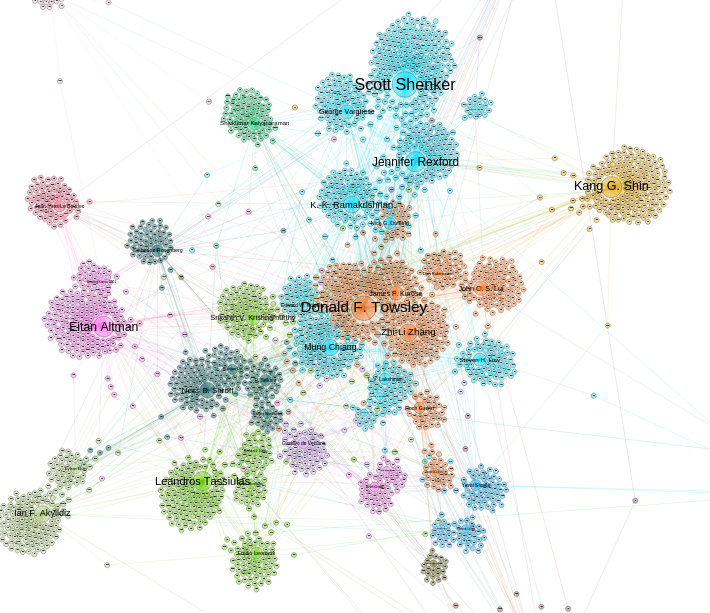
\includegraphics[scale=0.5]{img/ton}
    \caption{Graph of couauthorships with researchers from the sub-area of Computer Networking, using the venue TON as source of reputation.}
    \label{fig:ton}
\end{figure}

\begin{figure}[h]
    \centering
    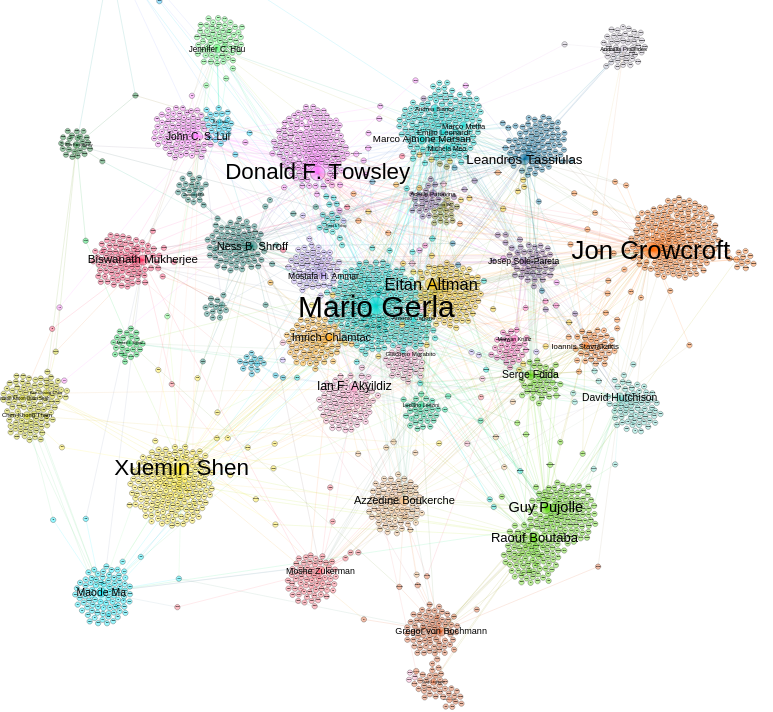
\includegraphics[scale=0.45]{img/cn}
    \caption{Graph of couauthorships with researchers from the sub-area of Computer Networking, using the venue Computer Networks as source of reputation.}
    \label{fig:cn}
\end{figure}


\begin{figure}[h]
    \centering
    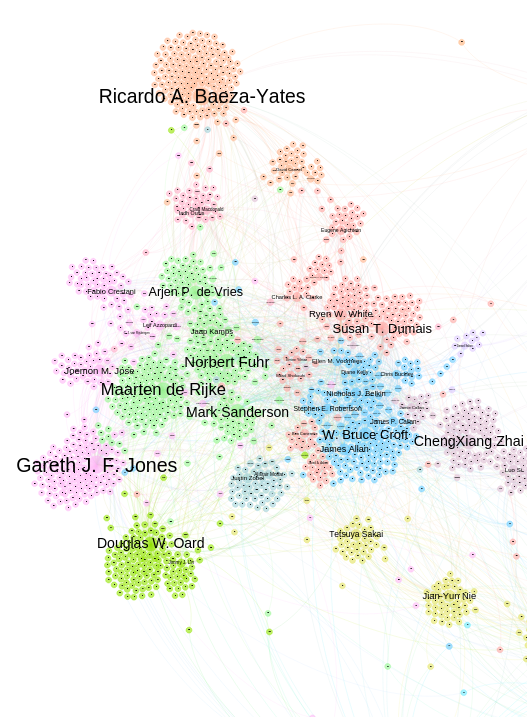
\includegraphics[scale=0.6]{img/sigir}
    \caption{Graph of couauthorships with researchers from the sub-area of Information Retrieval, using the venue SIGIR as source of reputation.}
    \label{fig:sigir}
\end{figure}

\begin{figure}[h]
    \centering
    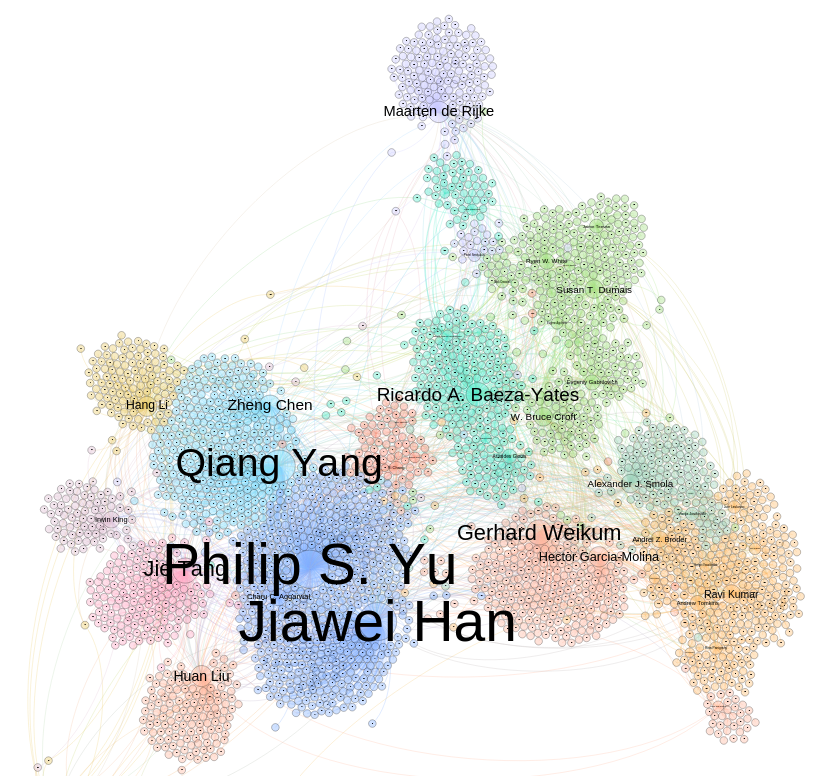
\includegraphics[scale=0.45]{img/wsdm}
    \caption{Graph of couauthorships with researchers from the sub-area of Information Retrieval, using the venue WSDM as source of reputation. }
    \label{fig:wsdm}
\end{figure}

%they create paths among components, they tend to connect themselves mostly with nodes of small degree values, decreasing the assertiveness of the network. Indeed, a senior researcher might tend to be a coauthor of a high number of students and young researchers, but also keep collaborations with other senior researchers from other groups.

% Machine Learning, key features
% 

\subsection{Next Steps}

The use of clustering methods is just an initial step to generate reputable sources in a sub-area. The goal is to rank venues, authors, and departments in a given sub-area by computing P-scores based on the reputable sources identified.

The framework we want to propose has multiple components between the initial input (reputation reference) and the final output (a ranking of venues, research groups, or individual researchers) . This implies that there are several decision points within the framework. Each of these points must be studied and tested before we choose a given strategy as a standard approach. Examples of questions which we should answer  in this framework are: i) How to select representative authors of a sub-area based only on a single publication venue of this sub-area? ii) Could we use the information provided by the resulting clusters as relevance feedback to the process (e.g. most centered clusters, largest clusters)? iii) Does the final result improve in quality if we use more than one publication venue as reputation source? If so, how many publication venues lead to the optimal result?

Also, we intend to test our strategies of ranking academic entities varying the method parameters of the algorithms. In this way, we want to check if our approach is robust enough to generate rankings of good quality -- even with perturbations on the data input -- and which are the more indicated values for the parameters and the reasons for that. Specifically, the reputation flow model allows us to increase or decrease the quantity of reputation that is transferred in each of the quadrants shown in section 2.3. %ref

With a stable ranking algorithm defined, we can make a characterization of sub-areas of Computer Science in Brazil and compare the Brazilian departments to other international departments. We could also analyze which Brazilian sub-areas should be highlighted and which must be updated in terms of scientific impact. Besides that, following the research questions we want to answer with this work, we can make initial experiments for the problem to find good references of reputation in any topic of study in any sub-area (e.g., ``land policies'', ``infectious diseases'', ``deep learning'', among others).

\section{Tasks and Dates}

\ \\

{\centering \begin{tabular}{| l | c | c | c | c | c | c | c | c |} \hline
\multicolumn{9}{| c |}{\textbf{\normalsize 2016 Schedule}} \\[2pt] \hline
Task                      &  May   &  Jun   &   Jul  &   Aug   &   Sep  &   Oct  &   Nov  &  Dec   \\ \hline
Thesis' project proposal  &   X    &        &        &         &        &        &        &        \\ \hline
Advisers assistant        &   X    &   X    &    X   &    X    &    X   &    X   &   X    &   X    \\ \hline
Experiments      &   X    &   X    &    X   &    X    &    X   &        &        &        \\ \hline
Writing                   &        &        &    X   &    X    &    X   &    X   &        &        \\ \hline
Defense                   &        &        &        &         &        &    X   &        &        \\ \hline
\end{tabular}}

\ppgccbibliography{masters}

\begin{appendices}
%\chapter{Um ap�ndice}
\end{appendices}	

\begin{attachments}
%\chapter{Um anexo}
\end{attachments}

\end{document}